\documentclass[10pt]{article}

% Set paper
\usepackage[a4paper,top=0.98in, bottom=0.98in, left=0.98in, right=0.98in]{geometry}

% The Calibri font is proprietary. The open source Carlito font is close enough.
% The 10pt font is scaled by 0.95 to get the required 9.5pt.
\usepackage{fontspec}
\defaultfontfeatures{Scale=0.95}
\linespread{1.09}
\setmainfont{Carlito}

\usepackage{graphicx}
\graphicspath{{figures/}}
\usepackage[table]{xcolor}
\usepackage[super]{natbib}
\usepackage{parskip}

%% remove the header for the bibliography section because it is already included as a section header
\renewcommand{\bibsection}{}
%% decrease whitespace between entries
\setlength{\bibsep}{2.0pt}
\usepackage{hyperref}

\usepackage{sectsty}
\usepackage{enumitem,amssymb}
\usepackage{bm}
\usepackage{pifont}
\usepackage{tabularx,tabu}
\usepackage{todonotes}

\usepackage{multirow}
%\usepackage{luacolor}
\usepackage{wrapfig}

%% Colors extracted from NWO's Word template
\definecolor{sectionblue}{RGB}{0, 139, 159}
\definecolor{headerblue}{RGB}{65, 81, 102}
\definecolor{tableblue}{RGB}{38, 97, 119}

\hypersetup{
    colorlinks=true,
    linkcolor=black,
    filecolor=magenta,      
    urlcolor=sectionblue,
    pdftitle={NWO VIDI 2021 proposal Your Name},
    }
\newlist{todolist}{itemize}{2}
\setlist[todolist]{label={\color{sectionblue}$\square$}}
% \newcommand{\cmark}{\ding{51}}%
\newcommand{\cmark}{$\checkmark$}%
\newcommand{\done}{\rlap{\color{sectionblue}$\square$}{\raisebox{2pt}{\large\hspace{1pt}\cmark}}\hspace{-2.5pt}}
\newcommand{\notdone}{{\color{sectionblue}$\square$}}

%% Correct style for section titles
\sectionfont{\normalfont\color{sectionblue}\fontsize{17}{17}\selectfont}  % sets colour of sections
\subsectionfont{\normalfont\color{sectionblue}\fontsize{13}{13}\selectfont}  % sets colour of sections

%% Font used in table headers
\newcommand{\tableheadfont}{\bfseries\fontsize{10}{10}\selectfont\leavevmode\color{tableblue}}

% Section numbering
\renewcommand\thesection{\arabic{section}.}
\renewcommand\thesubsection{\arabic{section}\alph{subsection}.}
\renewcommand\thesubsubsection{\arabic{section}\alph{subsection}\arabic{subsubsection}.}
\renewcommand{\theparagraph}{\arabic{section}\alph{subsection}\arabic{subsubsection}.\arabic{paragraph}.}
\setcounter{secnumdepth}{4}

%% Automatic word count. Only works if texcount is installed and write18 is enabled
%% (call lualatex with --enable-write18).

\newcommand{\wordcount}[1]{\input{|./seccount \jobname.tex '#1'}}
%% you can comment  the above and uncomment the command below to disable the word counting feature 
%\newcommand{\wordcount}[1]{tbd words}


\newtheorem{objective}{Objective}
\newcommand{\standout}[1]{\begin{objective} #1\end{objective}}


\begin{document}
	\noindent
	\begin{minipage}{.85\linewidth}
		\color{headerblue}
		{\rmfamily\fontsize{20}{20}\selectfont Grant application proposal form 2021}\\[0.3cm]
		{\rmfamily\fontsize{15}{15}\selectfont NWO Talent Programme -- Vidi scheme}\\[0.25cm]
		{\rmfamily\fontsize{11}{11}\selectfont
		Applied and Engineering Sciences\\
		Social Sciences and Humanities\\
		Science\\
		Health Research and Development}
	\end{minipage}%
	\begin{minipage}{.15\linewidth}
		
\includegraphics[height=3.5cm]{NWO_logo}
	\end{minipage}
	\section{Institution and field of research}
	
	\subsection{NWO domain}
	Science (ENW)\todo{adapt as needed}
	\subsection{Title of the research proposal}
	Your Brilliant Title
	\subsection{Summary (max 300 words)}
	Your summary

	%TC:ignore
	(\wordcount{Summary}\todo{Note: in the tex file you can see comments \%TC:ignore and \%TC:endignore which wrap around latex sections which shouldn't be counted in the word count})
	%TC:endignore
	\subsection{Keywords (max 5)}
	key words,..
	
	\subsection{Main field of research}
	\todo{Adjust the codes to your proposal}

	\begin{tabularx}{\linewidth}{|>{\cellcolor[gray]{0.95}}p{3.6cm}|X|}
		\arrayrulecolor[gray]{0.8}\hline
		\rowcolor[gray]{0.95}
		&Code/Field of research: \\\hline
		Main field of research: & 15.70.00   Geodesy, physical geography \\\hline
		Other field(s) of research  & 15.90.00     Earth sciences\\
        (if applicable): &15.60.00     Hydrosphere sciences\\
        &15.50.00     Atmosphere sciences\\\hline
	\end{tabularx}
	
	\subsection{Public summary}
	\noindent NL\\
	\begin{tabularx}{\linewidth}{|X|}
		\arrayrulecolor[gray]{0.8}\hline 
		\rowcolor[gray]{0.95} {\tableheadfont Short NL title} \\\hline
		\rowcolor[gray]{0.95} \textit{\textcolor{tableblue}{Dr. xxxxx  Faculteit ...., Universiteit ..}}\\\hline
		short NL public summary\\\hline
		\rowcolor[gray]{0.95}\textcolor{tableblue}{Wordcount:}\\\hline
	\end{tabularx}\\
	
	\noindent ENG\\
	\begin{tabularx}{\linewidth}{|X|}
		\arrayrulecolor[gray]{0.8}\hline 
		\rowcolor[gray]{0.95} {\tableheadfont Short EN title} \\\hline
		\rowcolor[gray]{0.95} \textit{\textcolor{tableblue}{Dr. xxxxx, Faculty ..., University ..}}\\\hline
		Short EN summary\\\hline 
		\rowcolor[gray]{0.95}\textcolor{tableblue}{Wordcount:}\\\hline
	\end{tabularx}\\
		
	\section{Research proposal}
	
	\subsection{A description of the proposed research}
		
	\subsubsection{Overall aim and key objectives}
	%% hyper links are not allowed so the NoHyper environment disables turning urls in clickable hyperlinks
	\begin{NoHyper}
	    The overall aim of this Vidi ..
	    %note: paragraphs will get a number
	    \paragraph{Scientific challenges..\\}
		In \citep{masson-delmotteClimateChange20212021}
	    

	    \subparagraph{subheader 1\\}
	    \paragraph{Originality and innovative character\\}
	     
	   

	\paragraph{Research Approach}

	\subparagraph{Subheader\\}
	
	
	\subsubsection{Research plan}
	\paragraph{Practical timeline over the grant period\\}
	\begin{figure}[h!]
            \centering
        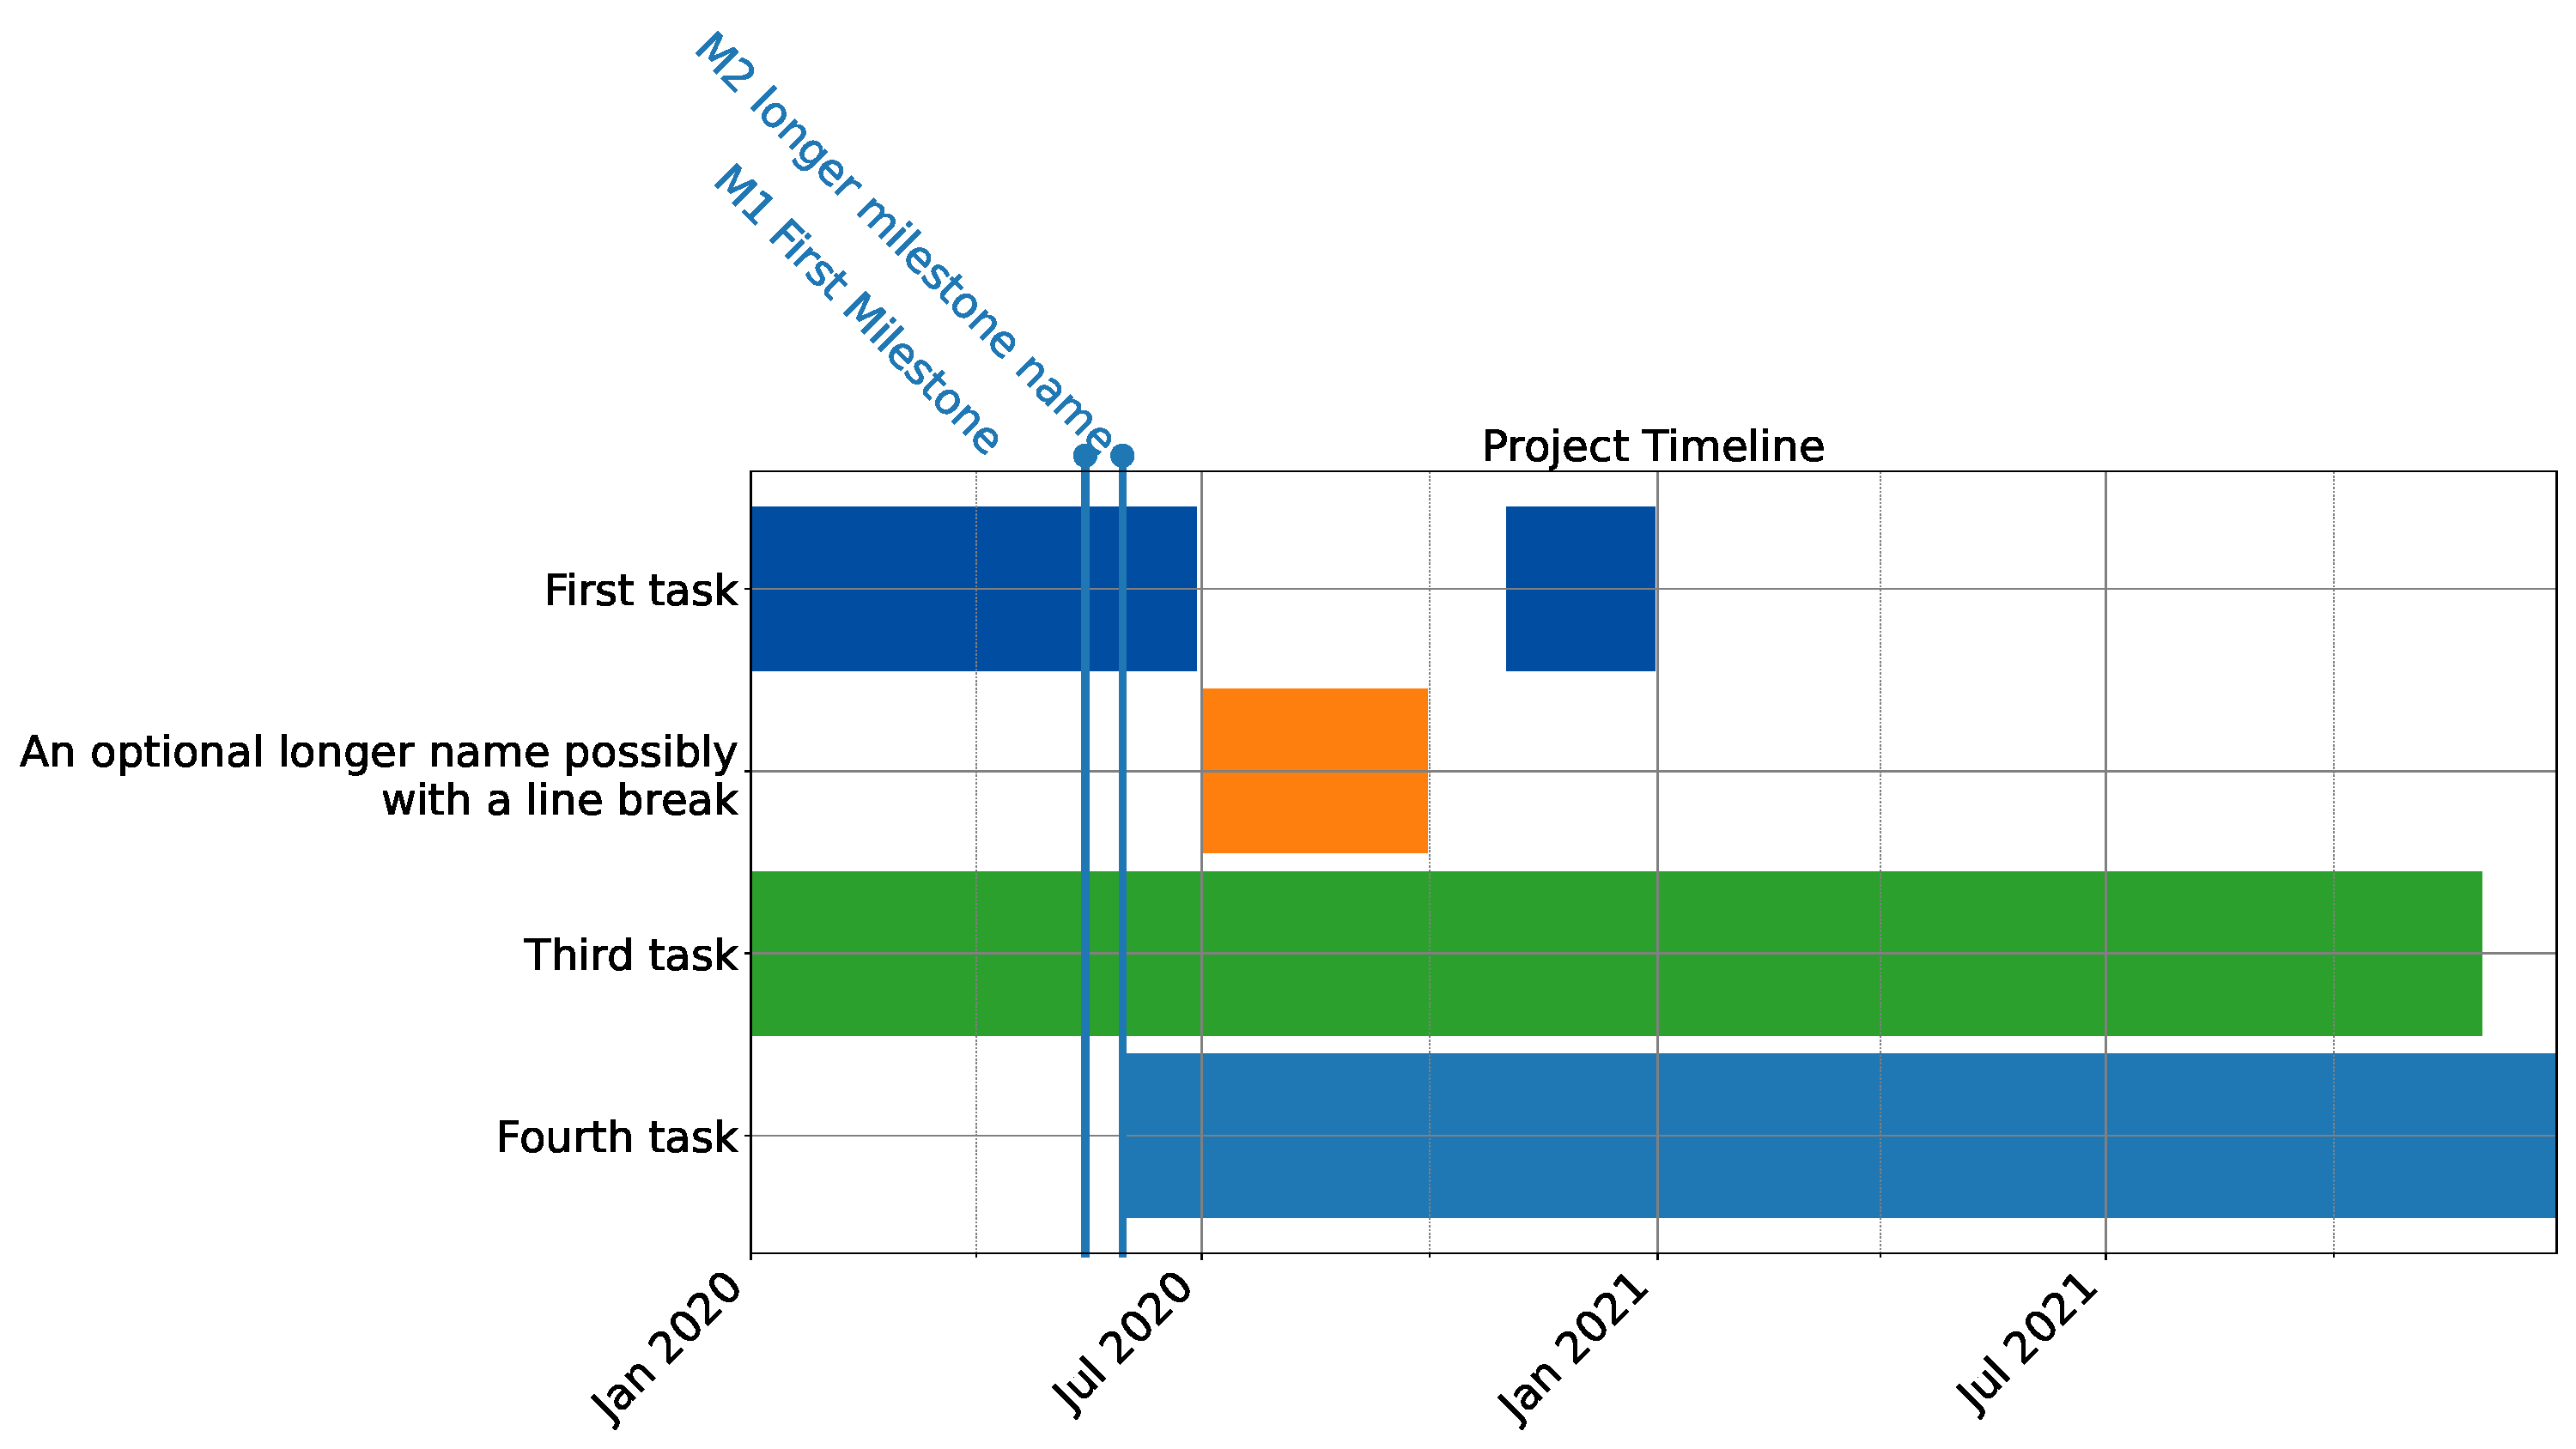
\includegraphics[width=0.95\textwidth]{figures/vidiGannt}
                \caption{The project will span 5 years...}
         \label{fig:gannt}
        \end{figure}
	\paragraph{Local, national and international collaboration\\}
	\paragraph{Methods, techniques and work plan for requested personnel\\}

	\subsubsection{Motivation for choice of host institute}

    \subsection{Scientific and/or societal impact of the proposed project (Knowledge utilisation)}
	    \textit{Scientific and societal impacts are of comparable focus}\todo{Choose your profile}\\

		
	\subsection{Number of words}
	
	\noindent
	Section 2a: \quad \wordcount{A description of the proposed research} \quad (max. 4,000 words/8 pages)\\
	Section 2b: \quad \wordcount{Scientific and} \quad (max. 1,000 words/2 pages)
	
	\subsection{Literature references}
    {\fontsize{8.5}{8.5}\selectfont
% 	\bibliography{roelofszotero}
	\bibliography{references}
	}
	
	\bibliographystyle{unsrtnat}	
	\subsection{Data management section}
	
	\begin{enumerate}
		\item Will data be collected or generated that are suitable for reuse?
		\begin{todolist}
			\item[\done] Yes: Then answer questions 2 to 4.
			\item No: Then explain why the research will not result in reusable data or in data that cannot be stored or data that for other reasons are not relevant for reuse.
		\end{todolist}
	    \item Where will the data be stored during the research?\\\todo{at argumentation to the bullet points}
    	\item After the project has been completed, how will the data be stored for the long-term and made available for the use by third parties? To whom will the data be accessible?\\
		\item Which facilities (ICT, (secure) archive, refrigerators or legal expertise) do you expect will be needed for the storage of data during the research and after the research? Are these available?\\
	\end{enumerate}
	\end{NoHyper}
	\section{Budget}
	
	\subsection{Budget}
	%The maximum amount of a Vidi grant is € 800,000, to be spent over a period of five years. If the proposed research is of shorter duration, the maximum grant amount will be reduced accordingly.
	
	\vspace{0.4cm}
	\noindent
	{\renewcommand{\arraystretch}{1.5}
	\begin{tabularx}{\linewidth}{|>{\cellcolor[gray]{0.8}\tableheadfont}X|l|l|l|l|l|l|l|l|l|}
		\arrayrulecolor[gray]{0.4}\hline
		\rowcolor[gray]{0.8} & \multicolumn{3}{c|}{\tableheadfont Description} & {\tableheadfont Year 1} & {\tableheadfont Year 2} & {\tableheadfont Year 3} &  {\tableheadfont Year 4} &  {\tableheadfont Year 5} &  {\tableheadfont Total} \\\hline
		\rowcolor[gray]{0.8} Staff & & {\tableheadfont FTE**} & {\tableheadfont Months} & & & & & & \\\hline
		WP* & Applicant & && €xxxxx & €xxxxx&€xxxxx &€xxxxx & €xxxxx&€xxxxxx\\\hline
		WP* &Phd 1 &&& & & & & &\\\hline
		WP* & && & & & & & &\\\hline
		NWP* & &  &  & & & & & & \\\hline
		\multicolumn{4}{|c|}{\cellcolor[gray]{0.8}\tableheadfont Total staff} &  &  &  & & &€xxxxxx\\\hline
		Equipment & \multicolumn{3}{l|}{\ldots} & & & & & & \\\hline
		Investments & \multicolumn{3}{l|}{\ldots}& & & & & & \\\hline
		Consumables & \multicolumn{3}{l|}{\ldots} & & & & & & \\\hline
		Travel & \multicolumn{3}{l|}{ } &  & & & & &  \\\hline
		Other & \multicolumn{3}{l|}{Other expenses}  & & & & & & \\\hline
		\multicolumn{4}{|c|}{\cellcolor[gray]{0.8}\tableheadfont Total Materials} & & & & & & €xxxxx\\\hline
		\multicolumn{4}{|c|}{\cellcolor[gray]{0.8}\tableheadfont Grand total} & & & & & &€xxxxxx \\\hline
	\end{tabularx}
	}
	\begin{itemize}
		\item[*]WP = Scientific staff; NWP = Non-scientific staff; please also list the nature of the post (for example PhD student or
		postdoc researcher)
		\item[**] Please list the time you will spend on your Vidi, including any FTE percentage that your host institution will pay of
		your salary for your work on this Vidi project. If your host institution pays for (part of) the time you spend on
		your Vidi, please include this information in section 3b. 
	\end{itemize}

	\subsection{Contributions `in kind'}

	{\renewcommand{\arraystretch}{1.5}
	\begin{tabularx}{\linewidth}{|X|X|X|}
		\arrayrulecolor[gray]{0.4}\hline
		\rowcolor[gray]{0.8} {\tableheadfont Contributing party} & {\tableheadfont Description } & {\tableheadfont Estimated value in euros} \\\hline 
	 & & €xx\\\hline
	\end{tabularx}
	}

	\subsection{Contributions `in cash'}

	{\renewcommand{\arraystretch}{1.5}
	\begin{tabularx}{\linewidth}{|X|X|X|}
		\arrayrulecolor[gray]{0.4}\hline
		\rowcolor[gray]{0.8} {\tableheadfont Contributing party} & {\tableheadfont Description } & {\tableheadfont Value in euros} \\\hline 
		& & €xx\\\hline
	\end{tabularx}
	}
	
	\subsection{Totals}
	{\renewcommand{\arraystretch}{1.5}
	\begin{tabularx}{\linewidth}{|p{3cm}|X|}
		\arrayrulecolor[gray]{0.4}\hline
		{\cellcolor[gray]{0.8}\tableheadfont Grand total} & €xxxxxx\quad (=3a) \\\hline 
		{\cellcolor[gray]{0.8}\tableheadfont Requested budget} & €xxxxxx \quad (=3a minus 3b and 3c) \\\hline 
	\end{tabularx}
	}

	\subsection{Additional grants for this project}
	Please include details of any additional (application for) funding for (part of) this research project, whether from NWO or from any other institution (e.g. ERC).
	Have you applied for any additional grants for this project either from NWO or from any other institution, 	and/or has the same idea been submitted elsewhere?
	\begin{todolist}
	\item[\done] No 
	\item Yes (please provide details)
	\end{todolist}

	
	\section{Curriculum Vitae}
	
	\subsection{Academic Profile}
	%TC:ignore
	%\begin{tabularx}{\linewidth}{|X|}
		%\arrayrulecolor[gray]{0.8}\hline
	%Provide a comprehensive narrative of your academic achievements, research focus, research agenda, position in your (inter)national academic field, motivation, and the academic and societal potential of your work. 
%(Max. 1.000 words)\\\hline
	    Wordcount:\wordcount{Academic Profile}\\%\hline
	%\end{tabularx}
    	%TC:endignore
	\begin{NoHyper}
	    \todo{Your narrative CV}
	\end{NoHyper}

	\subsection{Key output}
	%TC:ignore
	%\begin{tabularx}{\linewidth}{|X|}
		%\arrayrulecolor[gray]{0.8}\hline
	%Provide the references to your key output (max. 10) and add a motivation for the selection of each of these items. Please also number the items. You are allowed to use a hyperlink that refers to the article directly. You are not allowed to mention H-indexes, journal impact factors, or any type of metric that refers to the journal, publisher, or publication platform, rather than to the individual output item. For more information, see the Explanatory Notes. 
%(Max. 10 items. Min. 400 words - max. 700 words, excl. output titles and references to the output) \\\hline
	    %Wordcount:\wordcount{Key output}\\\hline
	%\end{tabularx}
	Wordcount: \wordcount{Key output}\\
	%TC:endignore
	\begin{enumerate}
		%TC:ignore
	    \item \label{ko:ky1}{\small Key output 1\\} 
		%TC:endignore
		{Explainer key output 1 }
		%TC:ignore
	    \item \label{ko:ky2} {\small Key Ouput 2\\}
		%TC:endignore
		{ Explainer Key output 2}
	\end{enumerate}
\section{Administrative details}
	\subsection{Personal details}

	\begin{tabularx}{\linewidth}{|>{\cellcolor[gray]{0.8}\tableheadfont}X|X|}
		\arrayrulecolor[gray]{0.4}\hline
		Title(s), initial (s), surname (s) & \\\hline 
		%Preferred language of correspondence (choose one): &\notdone Dutch   \done English \\\hline
	\end{tabularx}

	\subsection{Master's degree ('doctoraal')}
	\begin{tabularx}{\linewidth}{|>{\cellcolor[gray]{0.8}\tableheadfont}X|X|}
		\arrayrulecolor[gray]{0.4}\hline
		University/College of Higher Education: &  \\\hline 
		Main subject:&\\\hline 
	\end{tabularx}
	\subsection{Doctorate}
	
	\begin{tabularx}{\linewidth}{|>{\cellcolor[gray]{0.8}\tableheadfont}X|X|}
		\arrayrulecolor[gray]{0.4}\hline
		University/College of Higher Education: &  \\\hline
		Starting date: (dd/mm/yy):&\\\hline
		Date of PhD award (dd/mm/yy):&\\\hline
		Supervisor(s) ('Promotor(es)'):& \\\hline
		Thesis title:&\\\hline 
    \end{tabularx}
	
	\subsection{Prospective host institution} 
	\begin{tabularx}{\linewidth}{|>{\cellcolor[gray]{0.8}\tableheadfont}X|X|}
		\arrayrulecolor[gray]{0.4}\hline
		Host institution: & \\\hline
		Research group:& \\\hline
    \end{tabularx}
	
	\subsection{Work experience since completing your (first) PhD}
	List your appointments chronologically. The bottom row should contain your current position.	
	
	\noindent
	\begin{tabularx}{\linewidth}{|X|X|p{1cm}|X|X|}
		\arrayrulecolor[gray]{0.4}\hline
	\rowcolor[gray]{0.8}\tableheadfont Position & \tableheadfont Period
		(date-date) & \tableheadfont FTE &  \tableheadfont Position type
		(fixed term/permanent/ tenure-track/other) & \tableheadfont Institution \\\hline
	    &&&&\\\hline
	\end{tabularx}	
	
	\subsection{Months spent since completing your (first) PhD (include a calculation)}
	\begin{tabularx}{\linewidth}{|X|c|c|c|c|c|c|c|}
	    \arrayrulecolor[gray]{0.4}\hline
	    \rowcolor[gray]{0.8} \multicolumn{3}{|l|}{} & \multicolumn{5}{c|}{\tableheadfont Activities (fte)}\\\hline
	    \rowcolor[gray]{0.8} \tableheadfont Description/appointment	&	\tableheadfont period & \tableheadfont months& \tableheadfont	Research & \tableheadfont Education & \tableheadfont	Leave	& \tableheadfont Manag.& \tableheadfont Other\\\hline
	\multicolumn{2}{|l|}{Total in months}&&	 & &	 &		 &		\\\hline
	\end{tabularx}



	\begin{tabularx}{\linewidth}{|>{\cellcolor[gray]{0.8}\tableheadfont}X|X|}
		\arrayrulecolor[gray]{0.4}\hline
		\rowcolor[gray]{0.8} Experience & \tableheadfont Number of months \\\hline
		Research activities &  \\\hline
		Education &  \\\hline
		Leave & \\\hline
		Management tasks &  \\\hline
		Others (please specify): &  \\\hline
	\end{tabularx}

    %\vspace{1cm}\noindent
	\begin{tabularx}{\linewidth}{|X|}
		\arrayrulecolor[gray]{0.4}\hline
		\rowcolor[gray]{0.8} \tableheadfont If applicable: You may mention special circumstances (e.g. due to COVID-19) that account for a reduction in productivity\\\hline
		\\\hline
	\end{tabularx}
	
	\section*{Statements by the Applicant}
	\subsection*{Use of extension clause}
	If ‘yes’, (only) add the date of the confirmation e-mail (talent@nwo.nl, previously: vi@nwo.nl) that the extension was granted. An extension is only necessary if you exceed the year limit on the reference date.
	\begin{todolist}
		\setlength\itemsep{0em}
		\item[\done] No
		\item Yes, my extension was confirmed on: [date]
	\end{todolist}

	\subsection*{Ethical Aspects}

	\begin{tabularx}{\linewidth}{|>{\cellcolor[gray]{0.8}\tableheadfont}X|c|c|c|c|}
		\arrayrulecolor[gray]{0.4}\hline
		\rowcolor[gray]{0.8} & \tableheadfont Not applicable & \tableheadfont Not yet applied for & \tableheadfont Applied for & \tableheadfont Received \\\hline
		Approval from a recognised (medical) ethics review committee &\cmark &&&\\\hline
		Approval from an animal experiments committee &\cmark&&& \\\hline
		Permission for research with the population screening Act &\cmark&&& \\\hline
	\end{tabularx}	
	\subsection*{By submitting this form  declare that:}
    By submitting this form, I endorse the code of conduct for laboratory animals and the code of conduct for biosecurity/possibility for dual use of the expected results and will act accordingly, if applicable.
    \begin{todolist}
	\item[\done] I have completed this form truthfully\\By submitting this document, I declare that I satisfy the nationally and internationally accepted standards for scientific conduct as stated in the Netherlands Code of Conduct for Research Integrity 2018.
	\item[\done] I have submitted the completed and signed embedding guarantee
	\item[\done] I have submitted non-referees.*
	\item[\done] If applicable: I have included one or more authorised letters from the prospected host institution and/or a third party, guaranteeing to meet part of the costs of this research project.
    \end{todolist}
\begin{tabularx}{\linewidth}{|X|}
		\arrayrulecolor{sectionblue}\hline
{\tableheadfont Name:} \\\hline
{\tableheadfont Place:} \\\hline
{\tableheadfont Date:} \today\\\hline
\end{tabularx}
* You may indicate a maximum of three non-referees  in ISAAC or MijnZonMw. The non-referees will NOT be asked to assess your application. Please do not incorporate the names of your non-referees in this application form.\\
** Please refrain from using your first name to reduce gender effects.
\end{document}
